\documentclass[11pt]{article}

\usepackage{amsmath,amssymb,amsthm,enumerate,setspace,tabto,fancyhdr}
\usepackage{sectsty}
\fancyhf{}
\renewcommand{\headrulewidth}{0pt}
\usepackage{hyperref}
\hypersetup{
    colorlinks=true,
    linkcolor=blue,
    filecolor=magenta,      
    urlcolor=blue,
}
\usepackage{graphicx}
\usepackage[colorinlistoftodos]{todonotes}
\usepackage{float}
\usepackage{textcomp}
\usepackage[nobreak=true]{mdframed}
\def\coursenumber{EECS 149}
\def\class{Introduction to Embedded Systems}
\def\semester{Fall 2018}
\def\instructor{Prabal Dutta and Sanjit Seshia}
\def\title{Final Project}

\newskip\saveskip
\newskip\saveindent
\saveskip=\baselineskip

%%%%%% page headings

\def\foottext{\begin{footnotesize}\coursenumber, \semester, \title \hfill\qquad Detective Kobuki, page \thepage\end{footnotesize}}

\def\ps@myheadings{\let\@mkboth\@gobbletwo
\def\@oddfoot{\foottext}
\def\@evenfoot{\foottext}
\def\@evenhead{}\def\@oddhead{}}

\pagestyle{fancy}

%macros for use in assignments and exams

\sectionfont{\Large\fontfamily{lmdh}\selectfont}
\subsectionfont{\fontfamily{lmdh}\selectfont}

\def\tab{\hbox{\kern10pt}}

\textheight=9in
\textwidth=6.5in
\topmargin=-.75in
\oddsidemargin=0.25in
\evensidemargin=0.25in
\parindent=0pt
\parskip=5pt
\itemsep=-1pt
\floatsep 9pt plus 2pt minus 3pt
\intextsep 9pt plus 2pt minus 3pt
\textfloatsep=9pt plus 2pt minus 3pt
\renewcommand{\baselinestretch}{1.0}
\font\dunhd=cmdunh10 scaled \magstep3
\font\dunhc=cmdunh10 scaled \magstep2
\font\dunhb=cmdunh10 scaled \magstep1
\font\dunha=cmdunh10 scaled \magstep1
\date{}


\def\maketitle{%
 \begingroup
\hrule height6pt \vskip .7em
\makebox[1.5in][l]{\dunhb \coursenumber}
{\dunhb \class \hfill \ }
\vskip-0.1in 
\makebox[1.5in][l]{\dunhb \semester}
{\dunhb \instructor \hfill \dunhd \title \par} 
\vskip 0.6em
\hrule height6pt 
 \par
 \vskip .5em
 \thispagestyle{fancy}
 \endgroup
 \setcounter{footnote}{0}
 \let\maketitle\relax
}


%%%%%% additional symbols or names for them

\def\ceil#1{\lceil #1 \rceil}
\def\floor#1{\lfloor #1 \rfloor}

\def\N{\mathbb{N}}
\def\R{\mathbb{R}}
\def\Q{\mathbb{Q}}
\def\Z{\mathbb{Z}}
\def\O{\mathit{O}}
\def\qed{$\Box$}

\cfoot{\foottext}


\begin{document}

\maketitle

\section{Ultrasonic}
We make the ultrasonic sender and receiver by modifying existing ultrasonic range finder in the following ways:

\subsection{Sender}
To use an ultrasonic range finder as a beacon, simply trigger it at a desired interval, ignoring any response from the range finder. The highest possible trigger frequency is 30 Hz.

\subsection{Receiver}
The ultrasonic range finder will not give any response if not triggered first. We don't want to trigger it, because if we trigger it, it would send out an ultrasonic burst of its own, which could interfere with the bursts from the beacon. We worked around this problem by tapping into the receiver on board the range finder. An abstracted diagram of the range finder schematic is as follow:
\begin{figure}[H]
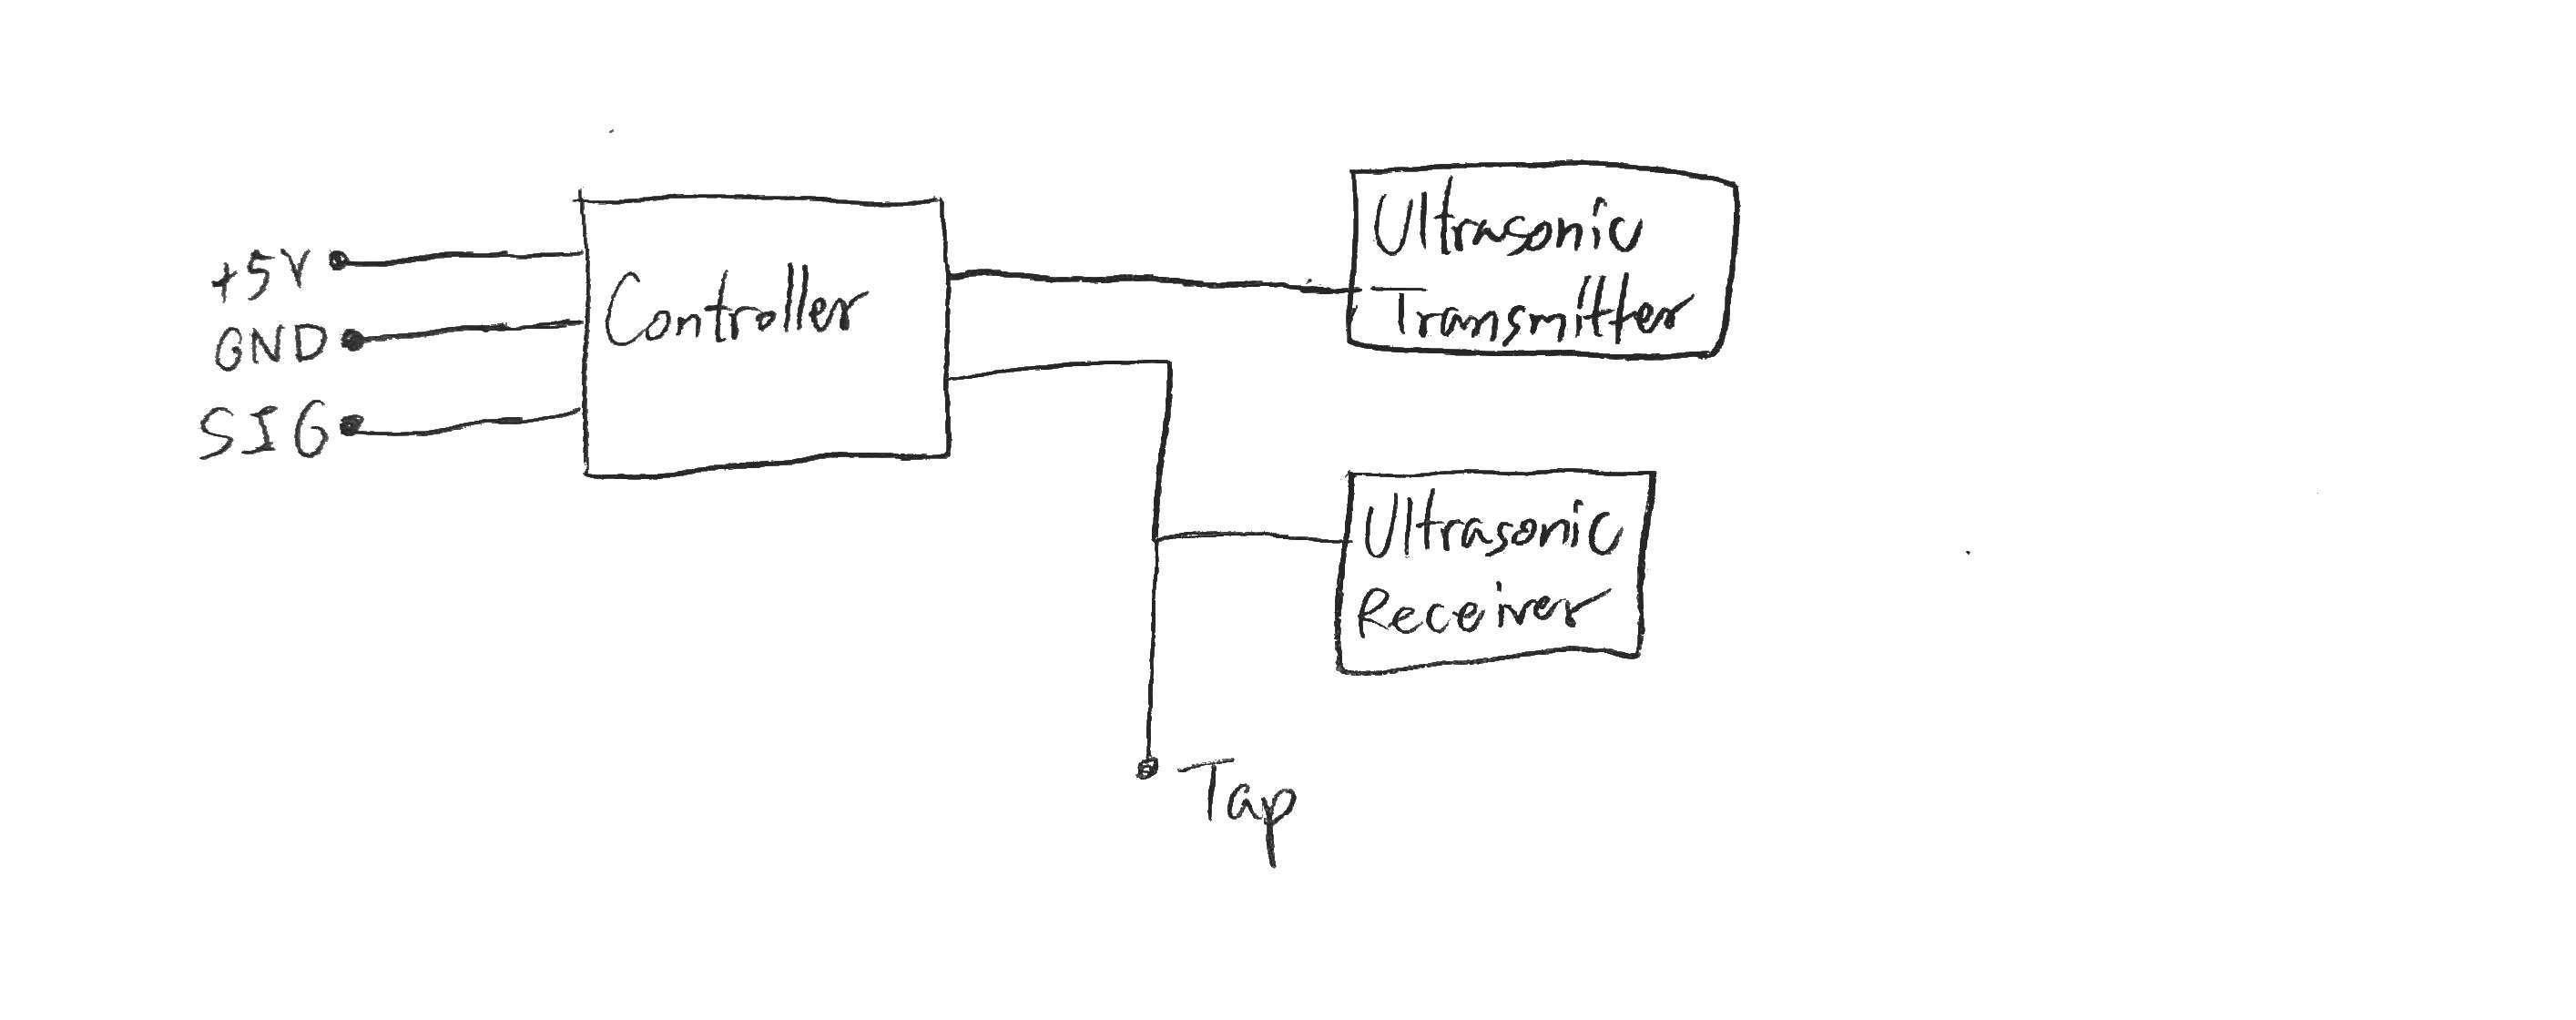
\includegraphics[width=\textwidth]{./assets/ultrasound_ranger_abstracted.jpg}
\caption{\label{fig:tapped}Tapped}
\end{figure}

The tapped signal is then fed to a comparator, then feed into a GPIO pin of the Buckler
\begin{figure}[H]
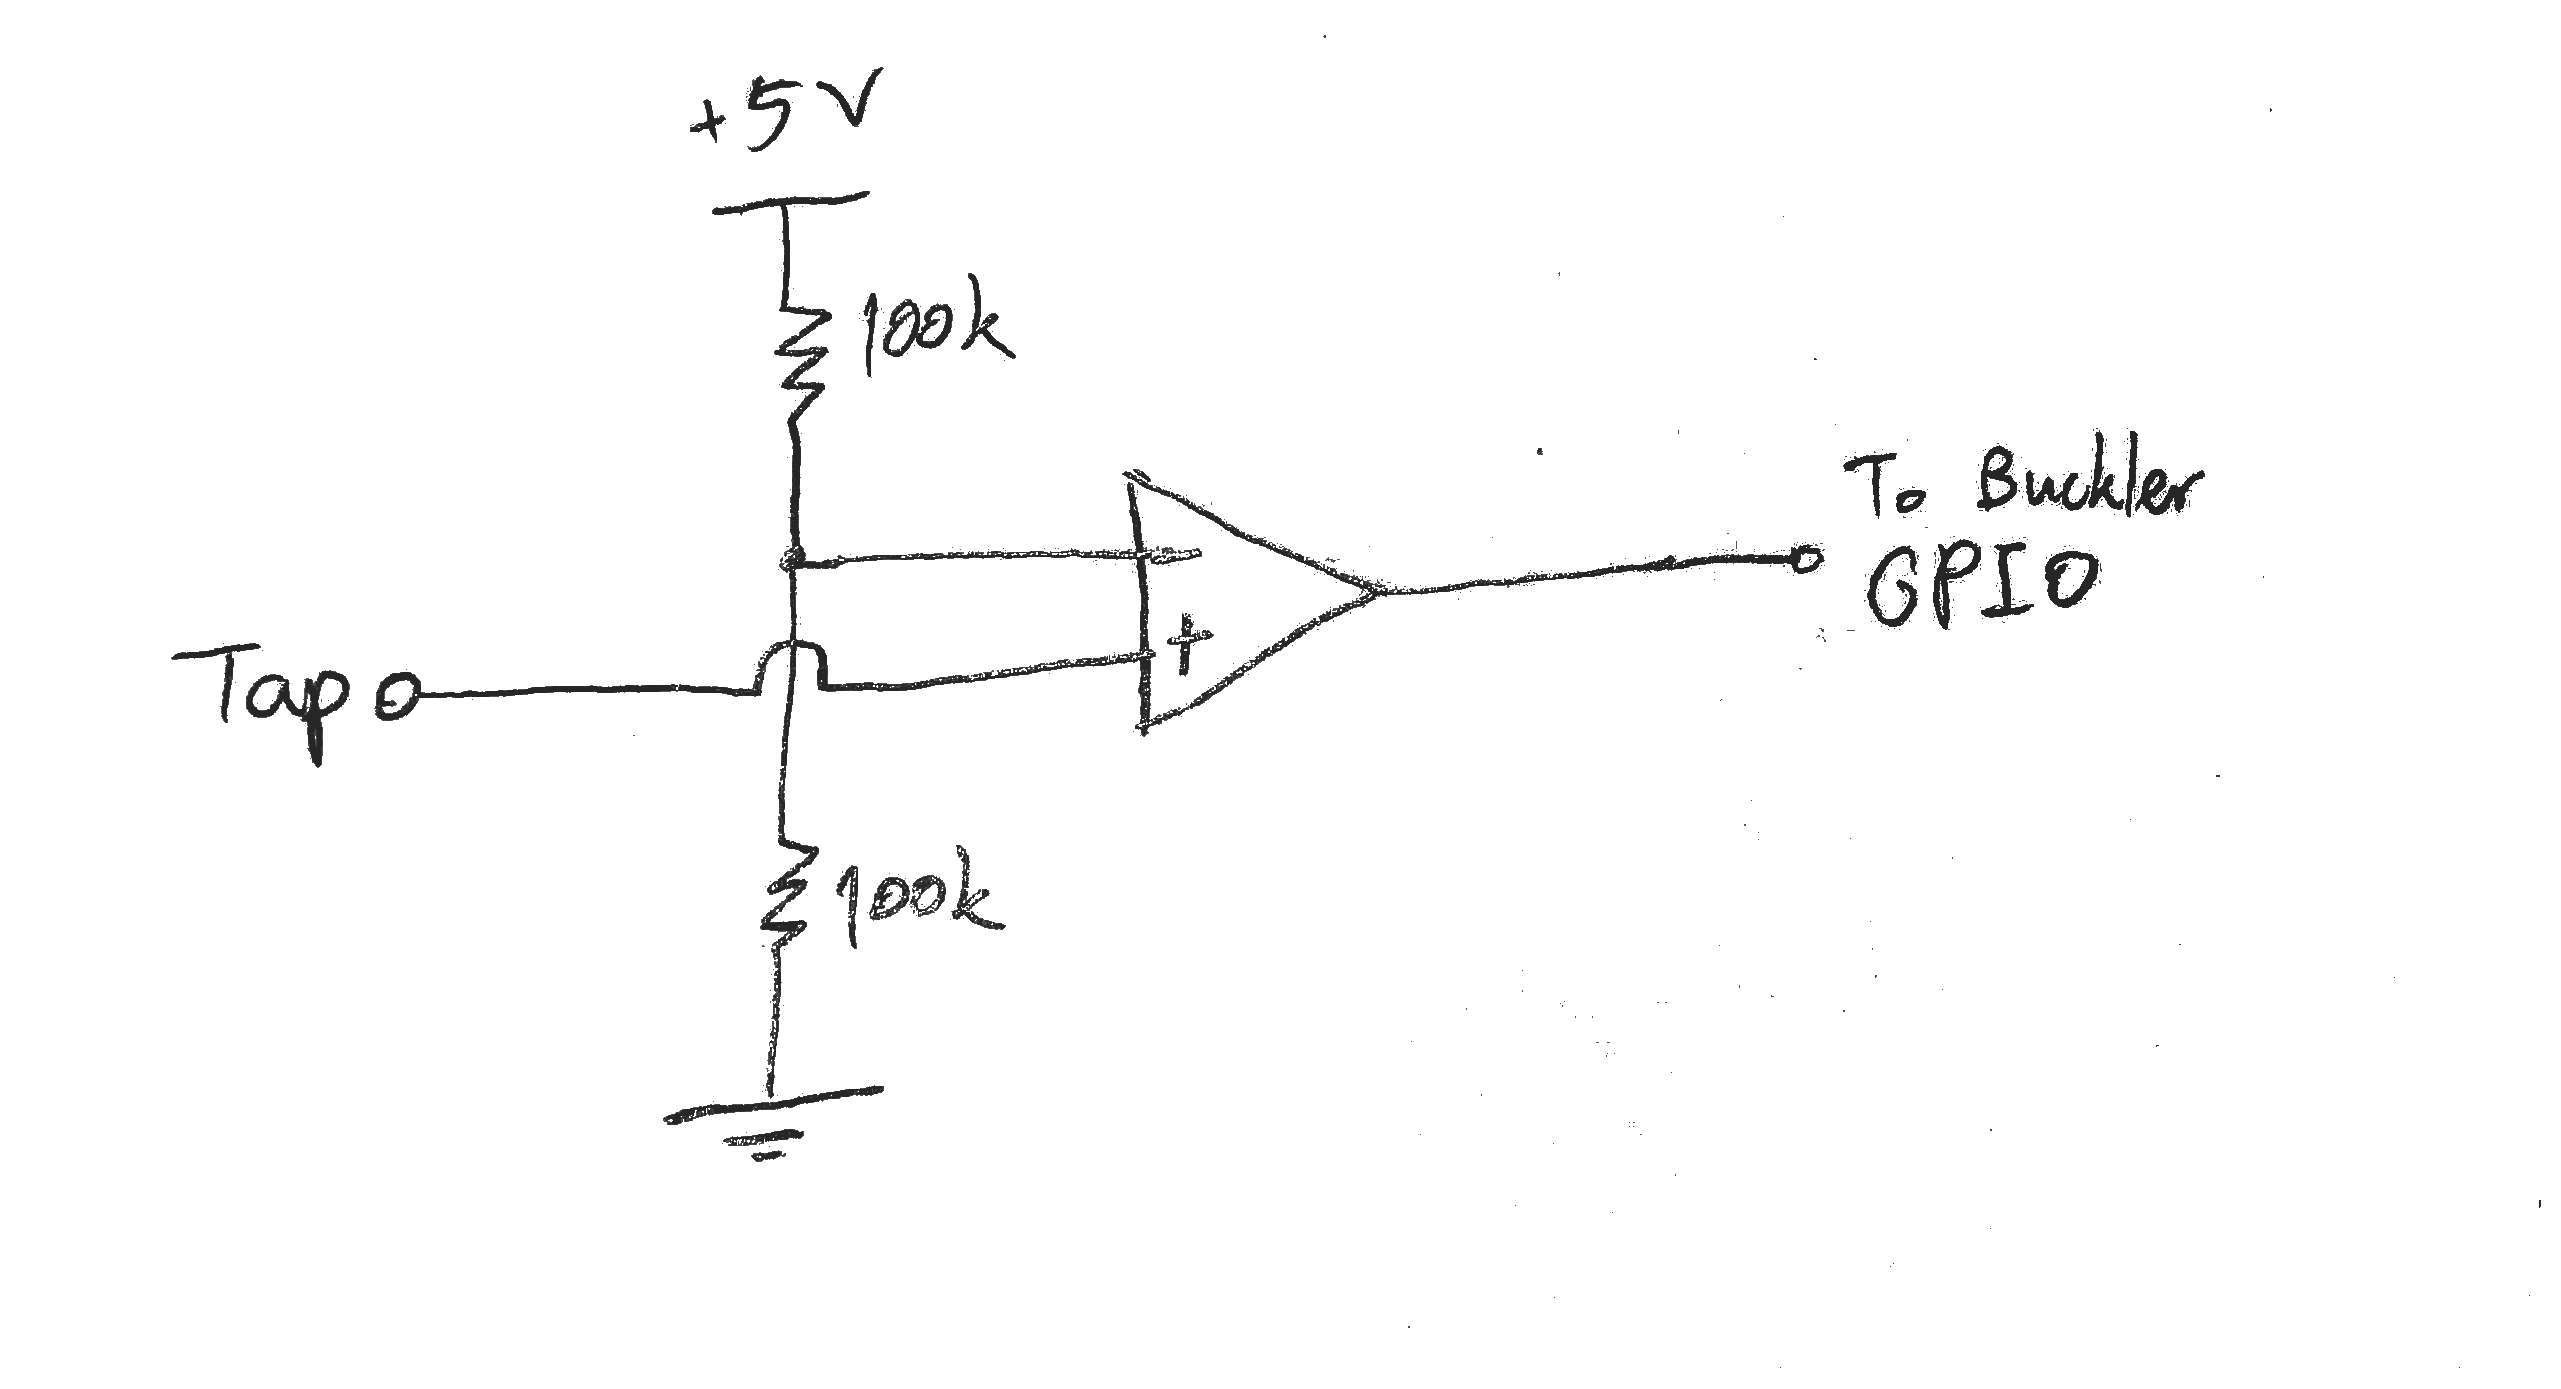
\includegraphics[width=.8\textwidth]{./assets/comparator.jpg}
\caption{\label{fig:comparator}comparator}
\end{figure}




\end{document}
